\documentclass[12 pt, a4paper]{article} %E aceptable tamen 11pt
%\usepackage[galician]{babel}\decimalpoint  %Para Galego
\usepackage[spanish]{babel}  %Para Castelan
%\usepackage[english]{babel}\decimalpoint    %Para Ingles
\usepackage[utf8]{inputenc} %acentos e caracteres para Windows & Linux         
\usepackage[T1]{fontenc}
\usepackage{graphicx}
\usepackage{color}
\usepackage{tikz}
\usepackage{anysize}
\usepackage{multicol}
\usepackage{bm}
\usepackage{textcomp}
\usepackage{eurosym}
\usepackage{amsthm}
\usepackage{amsmath}
\usepackage{amsfonts}
\usepackage{amssymb}
\usepackage{lineno}
\usepackage{epstopdf}
\usepackage{fancyhdr}
\usepackage{subfigure}
\usepackage{float}
\usepackage[square, numbers]{natbib}
\usepackage{longtable}
\usepackage{multirow}
\usepackage{array}
\usepackage{tabularx}
\usepackage[linkcolor=blue,colorlinks,]{hyperref}
\usepackage[all]{hypcap}
%\usepackage{lipsum}
\usepackage{mathdots}
\usepackage{braket}
\usepackage{yhmath}
\usepackage{cancel}
%\usepackage{siunitx}
\usepackage{gensymb}
\usepackage{booktabs}

\usetikzlibrary{fadings}
\usetikzlibrary{patterns}

\marginsize{1.5cm}{1.5cm}{2cm}{2cm} % MÁRGENES: Izq, Der, Sup, Inf.

\parindent=0mm %sangría
\parskip=3mm   %separacion entre parrafos
\usepackage{gensymb}

\numberwithin{equation}{section}
\numberwithin{figure}{section}
\numberwithin{table}{section}

\renewcommand{\spanishtablename}{Tabla} %Denominacion para tablas
\renewcommand{\spanishabstractname}{} %Denominacion para el abstract
\renewcommand{\spanishrefname}{Referencias} %Denominacion para las referencias
\renewcommand{\spanishfigurename}{Figura} %Denominacion para imagenes
\renewcommand{\spanishchaptername}{} %Denominacion para capitulos
\renewcommand{\spanishcontentsname}{Índice} %Denominacion para el indice

\marginsize{1.5cm}{1.5cm}{2cm}{2cm} % MÁRGENES: Izq, Der, Sup, Inf.

\definecolor{usc}{RGB}{15,41,118}
\definecolor{grise}{RGB}{234, 236, 240}
\newcommand{\abs}[1]{\lvert#1\rvert}

\newcommand{\vect}[1]{\boldsymbol{\mathbf{#1}}}


\begin{document}
	\pagenumbering{Roman}
	%%%%%%%%%%%%%%%%%%%%%%%%%%%% TITULO %%%%%%%%%%%%%%%%%%%%%%%%%%%%%%%%%%%%%%%%%%%%%%%%%%%%%%%
	\pagestyle{empty}
	
	\newcommand\TituloDoTraballo{Caracterización de la emisión en radio en cascadas atmosféricas iniciadas por
		neutrinos tau de muy altas energías en detectores a gran altitud}  % <-- Titulo tal como vai aparecer na portada externa e na interna. Debe coincidir co titulo subido a secretaria virtual no momento do deposito da memoria/solicitude de defensa. Non ten por que coincidir co titulo do proxecto do traballo (o titor debe incluir no seu informe o seu acordo co titulo final). O mais adecuado e que o titulo na portada este no idioma do texto principal da memoria. Tamen pode cambiarse de idioma do resto do contido da portada.
	
	\newcommand\EspecialidadeMaster{Especialidad en Física Nuclear y de Partículas}  % <-- Deixar valeiro no caso de TFG, e decir introducir {}. No caso de TFM, e IMPORTANTE que conste: Esta considerado un requisito para obter a especialidade da titulacion do master que a devandita especialidade conste no TFM,  sucedendo que na implementacion informatica da USC ao facer a solicitude de defensa de TFM na secretaria virtual a unica opcion onde introducir a especialidade e no propio campo do titulo do traballo. Por eso, a mencion de especialidade debe facerse como unha addenda ao titulo de TFM, a modo de subtitulo - en particular, na secretaria virtual, este subtitulo ou mencion a especialidade debe incluirse no mesmo campo informatico do titulo de TFM (por exemplo introducir no campo titulo do TFM "Estudio de superconductores ultrarelativistas. Especialidad en Fisica Fundamental." Asi vai aparecer tamen no expediente academico do estudante.)
	
	\newcommand\DataDefensa{Julio 2022} %<-Mes e ano da presentacion
	
	\begin{center}
		%{\sc\large\color{usc} \sc Universidade de Santiago de Compostela}
		\vspace{3em}
		
\includegraphics[width=10em]{figures/USC.png}
		\hspace{1cm}
		\begin{tabular}[b]{c}
			{\large\color{usc} \sc Facultad de Física} \vspace{0.5em}\\
			{\large\color{usc} \sc Grado en Física } \vspace{0.5em}\\  %<-- Ou Master
			{\large\color{usc}  Curso 2021-22} \vspace{0.5em}\\%Actualizar curso!
			{\Large\color{usc} \sc Trabajo de Fin de Máster} %<-- Ou Master
		\end{tabular}
		
		
		
		\vspace{3cm}
		\rule{65mm}{0.2mm}\\
		\vspace{1cm}
		
		{\sc\LARGE \TituloDoTraballo}
		
		{\sl\large \EspecialidadeMaster}
		
		
		
		\vspace{0.5cm}
		\rule{65mm}{0.2mm}\\
		\vspace{2cm}
	\end{center}
	
	
	\begin{tabular}{l}
		{\sl\large Autor:} \\
		{\bf\Large Sergio Cabana Freire} % nome e apelidos do estudante
		\vspace{1em}\mbox{} \\
		%
		{\sl\large Tutor:} \\
		{\bf\large Jaime Álvarez Muñiz} \\
		{\sl\large Departamento de Física de Partículas \& IGFAE}
		\vspace{1em}\mbox{} \\
		%
	\end{tabular}
	
	
	
	\mbox{}
	\mbox{}\hfill{\large \DataDefensa} \vspace{1cm}
	\begin{center}
	\noindent{\tiny El autor autoriza la consulta y empleo de esta memoria para uso acad\'emico y de investigaci\'on (autorizaci\'on detallada en las p\'aginas interiores).}
	\end{center}
	
	
	\clearpage
	\mbox{}
	\clearpage %fin portada externa, inicio portada interna%%%%%%%%%%%
	
	
	\mbox{}\\
	Facultad de F\'{\i}sica\\
	Grado en F\'{\i}sica \\  
	Curso 2021-22\\%Nota: actualizar curso
	{\sc Trabajo de Fin de Máster}\vspace{3cm}\\
	%
	{\sc\LARGE \TituloDoTraballo}\vspace{1cm}\\
	{\sl\large \EspecialidadeMaster}\vspace{2cm}\\
	%
	{\sl Autor:} {\bf Sergio Cabana Freire}\\ % nome e apelidos do estudante
	{\sl Tutor:} {\bf Jaime Álvarez Muñiz}, {\sl Departamento de Física de Partículas (USC) \& Instituto Galego de Física de Altas Enerxías (IGFAE)}\\
	\vspace{1cm}\\
	%
	%Opcionalmente, inclu\'{\i}r aqu\'{\i}  li\~nas de agradecementos a outras persoas que colaborasen, referencias a financiaci\'on econ\'omica, notas sobre patentes ou publicaci\'ons de traballos derivados do traballo, ou calqueira outra informaci\'on complementaria de contextualizaci\'on xeral do traballo que considere convinte.
	
	\mbox{}
	
	\mbox{}\hfill{Data de presentaci\'on: \DataDefensa}
	
	
	\clearpage
	%%%%%%%%%%%%%%%%%%%%%%%%%%%%%%%%%%%%%%%%%%%%%%%%%%%%%%%%%%%%%%%%%%%%%%%%%%%%%%%%%
	
	%%%%%%%%%%%%%%%%%%%%%%%%%%%%%%%%%%% DECLARACIONES %%%%%%%%%%%%%%%%%%%%%%%%%%%%%%%
	\thispagestyle{empty}
	\pagebreak
	
	{\sl Declaraci\'on firmada por el autor de la originalidad del trabajo}
	
	El autor del trabajo declara que e presente es un trabajo original. Autoriza asimismo al control por personal de la Universidade de Santiago de Compostela de la mencionada originalidad, eventualmente mediante el empleo de bases de datos y la inclusi\'on en ellas.
	
	En Santiago de Compostela, a X de julio de 2022. Firmado,\vspace{3cm}
	
	
	{\sl Autorizaci\'on del autor a la difusi\'on del trabajo}
	
	 El autor autoriza a la difusi\'on del trabajo a los efectos considerados en los vigentes reglamentos de TFG y TFM de la Universidade de Santiago de Compostela (Artículo 11.3) y de TFM del M\'aster en F\'{\i}sica (Artículo 33), entendiendo que esta autorizaci\'on no infl\'uye en la propiedad intelectual del trabajo ni a la posibilidad de publicar el mismo total o parcialmente por otros medios. Autoriza asimismo a que la Facultad de F\'{\i}sica de esa Universidad disponga de copia electr\'onica del trabajo para su archivo, consulta y empleo para usos acad\'emicos y de investigaci\'on con la menci\'on espec\'{\i}fica al autor. 
	
	En Santiago de Compostela, a X de julio de 2022. Firmado,\
	
	\thispagestyle{empty}
	\pagebreak
	%%%%%%%%%%%%%%%%%%%%%%%%%%%%%%%%%%%%%%%%%%%%%%%%%%%%%%%%%%%%%%%%%%%%%%%%%%%%%%%%%

	%%%%%%%%%%%%%%%%%%%%%%%%%%%%%%%%%%%%%%%% ABSTRACTS %%%%%%%%%%%%%%%%%%%%%%%%%%%%%%%%%%
	\thispagestyle{empty} %%<- poner en mas paginas si los resumenes ocupan varias (elimina la numeracion de la pagina actual)
	\pagebreak
	
		\begin{flushleft} \hyphenpenalty=10000\exhyphenpenalty=10000 {\bf $\bullet$ Resumen:\;\;}
		%
		Aqu\'{\i} va el resumen en castellano. El orden de los idiomas puede cambiarse a voluntad. Tambi\'en (y aunque la hoja de res\'umenes no contabiliza para el n\'umero l\'{\i}mite de p\'aginas, ver secci\'on \ref{quecontabiliza} de este documento) puede  reducirse, si se desea, el tama\~no de letra de los res\'umenes en los dos idiomas que no sean el usado  en el texto principal de la memoria (por ejemplo, anteponiendo \verb \footnotesize{}  al texto). % anteponiendo \footnotesize{} al texto, por ejemplo
		%
	\end{flushleft}\mbox{}

	\begin{flushleft} \hyphenpenalty=10000\exhyphenpenalty=10000 {\bf $\bullet$ Resumo:\;\;}
		%
		Aqu\'{\i} vai o resumo en galego. Debe coincidir co introducido na secretar\'{\i}a virtual no momento do dep\'osito da memoria final e solicitude de defensa. Dado que a aplicaci\'on inform\'atica de secretar\'{\i}a virtual non admite calqueira caracter, o regulamento permite introducir nela representaci\'ons alternativas dos caracteres problem\'aticos (por exemplo introducir gamma en vez de $\gamma$, introducir YBa2Cu3O(7-delta) en vez de \mbox{YBa$_2$Cu$_3$O$_{7-\delta}$}, etc.). Non ten por qu\'e coincidir co resumo do proxecto de TFG/TFM que foi feito no momento da asignaci\'on de traballo e titor (entendendo que o titor da o visto bo no seu informe final). Ten que haber resumos en (como m\'{\i}nimo) galego, castel\'an e ingl\'es, cada un de 300 palabras m\'aximo.
		%
	\end{flushleft}\mbox{}
	
	
	\begin{flushleft} \hyphenpenalty=10000\exhyphenpenalty=10000 {\bf $\bullet$ Abstract:\;\;}
		%
		The abstract goes here.
		%
	\end{flushleft}\mbox{}
	%%%%%%%%%%%%%%%%%%%%%%%%%%%%%%%%%%%%%%%%%%%%%%%%%%%%%%%%%%%%%%%%%%%%%%%%%%%%%%%%%%%%%
	%\clearpage
	%\include{capitulos/resumo} % paxina de resumo e agradecementos. Débese ter en conta o idioma seleccionado para o documento
	
	\clearpage
	\pagestyle{fancy}
	\fancypagestyle{plain}
	\lhead{}
	\chead{}
	\rhead{}
	\renewcommand{\headrulewidth}{0.1pt}
	\lfoot{} 
	\cfoot{\thepage}
	\rfoot{} 
	\renewcommand{\footrulewidth}{0pt}
	
	\pagenumbering{arabic}\setcounter{page}{1}
	\tableofcontents
	\clearpage
	
	%%%%%%% Incluimos as seccións que sexan necesarias
	\section{Introducción}\label{sec1}
	Comentar un poquito de rayos cosmicos, flujo escaso a altas energias -> EAS. 
	
	Comentar importancia de neutrinos en astronomia y astrofisica, problemas para detectar
	
	Detectores suelo, Cerenkov, fluerescencia, ... Radiodeteccion de EAS como otra opcion. Posibilidad de neutrino tau cascada hacia arriba (Tierra como blanco)
	
	\begin{figure}[H]
		\centering
		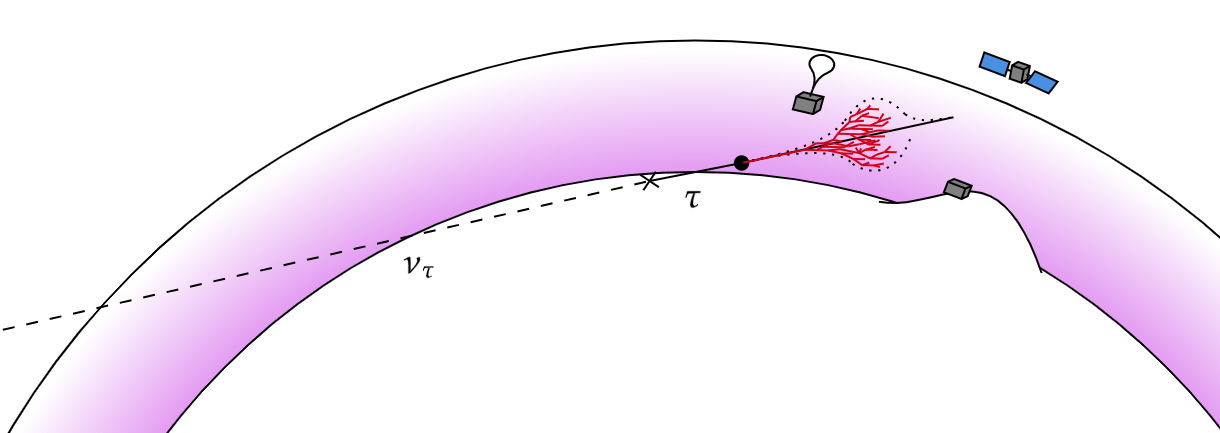
\includegraphics[width=.85\linewidth]{figures/shower_up}
		\caption{Idea de detección}
		\label{shower_up}
	\end{figure}
	\clearpage
	\section{Cascadas atmosféricas}\label{sec2}
%	Fisica, conceptos, etc
%	
%	Comentar AIRES
%	
%	Meter simulaciones de desarrollo UG, CompUGDG

Las cascadas atmosféricas, como hemos visto, representan la opción más importante para lograr estudiar la radiación cósmica mas energética. Debido a los escasos flujos ($<1\,\mathrm{m^{-2}y^{-1}}$ a partir de $E=10^{15}\,\mathrm{eV}$), la detección directa de estas partículas, por ejemplo en detectores situados fuera de la atmósfera, se hace inviable. Por ello, el estudio de la radiación cósmica en esta región de energías se realiza observando las consecuencias de las interacciones de estas partículas en la atmósfera. 

\subsection{Desarrollo de cascadas en la atmósfera}\label{sec21}

Cuando un rayo cósmico de muy alta energía (por ejemplo un protón) llega a las capas superiores de la atmósfera e interacciona con la materia presente en el medio, producirá un número elevado de partículas secundarias, a su vez de altas energías, que volverán a generar más partículas sucesivamente. De este modo, se desarrolla una \textit{cascada} de partículas propagándose a través de la atmósfera, en el que el número de partículas continúa aumentando progresivamente, hasta que la energía de las partículas no es suficiente para mantener el crecimiento (i.e., se alcanza un máximo del desarrollo). Gracias al elevado número de partículas producidas en esta clase de eventos (hasta $10^{11}$ para las partículas primarias más energéticas), su estudio es posible mediante diversas técnicas (detectores de partículas a nivel de suelo, estudio de la fluorescencia provocada por las partículas provocadas en la atmósfera, medidas de la radiación \v{C}erenkov, ...). En cierto modo, la atmósfera actúa como un calorímetro que permite extraer información acerca de la energía y dirección de llegada del rayo cósmico primario, a partir de la deposición de energía en el medio, en forma de una cascada atmosférica.

No obstante, usar la atmósfera como medio de detección tiene, evidentemente, las desventajas de que se trata de un medio inhomogéneo, ya que la densidad de la misma decrece con la altitud, $\rho = \rho(h)$. Como ejemplo, uno de los modelos más simples para la dependencia de la densidad con la altura es un decrecimiento exponencial:
\begin{equation}
	\rho(h)=\rho_0\exp\left(-h/h_0\right)\; \;;\;\;\text{donde}\;\rho_0\sim 10^{-3}\,\mathrm{g/cm^3}\;\text{y}\;h_0\sim8\,\mathrm{km}\label{ec21}
\end{equation}

Naturalmente, este hecho tendrá consecuencias importantes en el desarrollo de la cascada. Fundamentalmente, el efecto se deberá a que, a mayor densidad, mayor probabilidad de interacción para las partículas producidas. Para tener en cuenta esta cuestión, gran parte de la discusión que haremos acerca del desarrollo de cascadas atmosféricas no se hará en términos de distancias, sino de cantidad de materia atravesada o \textit{profundidad}, $X$. Dicha profundidad puede medirse en la dirección vertical ($X_v$) o a lo largo del eje del desarrollo de la cascada (Fig. \ref{shower_params}):
\begin{equation}
	X_v(h)=\int_{h}^\infty\rho(h')dh'\;\;;\;\;X_s(h,\theta)=\int_{h}^\infty\rho(h')dl=\int_h^{\infty}\frac{\rho(h')dh'}{\sqrt{1-\frac{R_T^2\sin^2{\theta}}{\left(R_T+h'\right)^2}}}\label{ec22}
\end{equation}
Gracias a estas definiciones, podremos estudiar el desarrollo de cascadas en términos de magnitudes que inmediatamente incorporan la inhomogeneidad de la atmósfera, por lo que no profundizaremos más en los modelos que describen la atmósfera y pasaremos a cuestiones de mayor interés para el objetivo de este trabajo.

\begin{figure}[H]
	\centering
	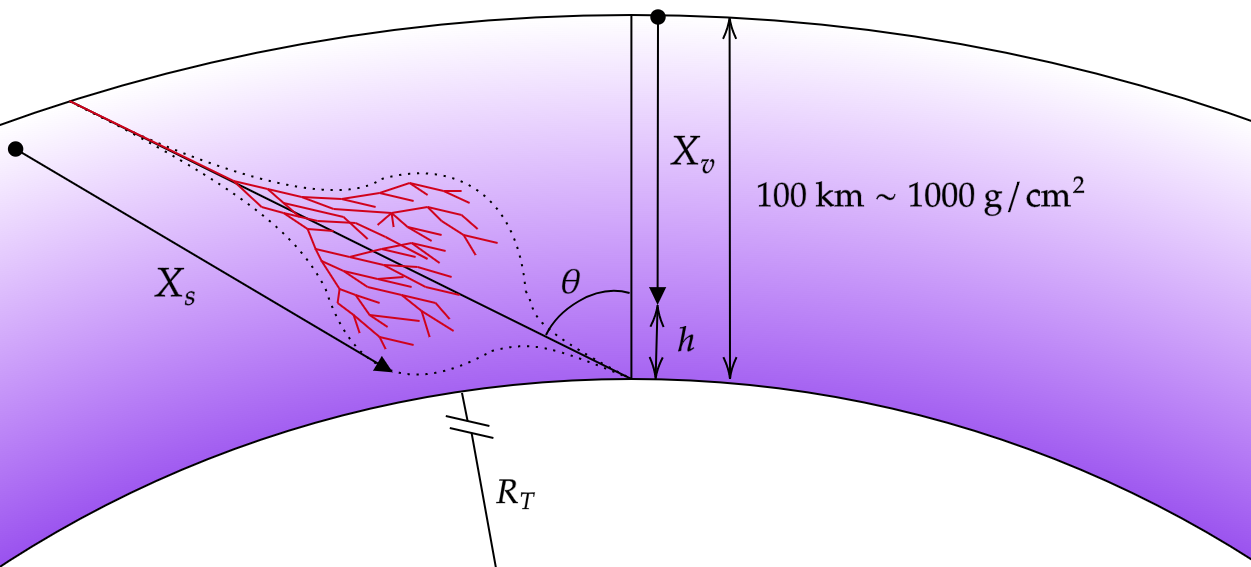
\includegraphics[width=.7\linewidth]{figures/cascadas/shower_params}
	\caption{Esquema de una cascada atmosférica \textit{al uso}. Definición de profundidad vertical e inclinada (\textit{slanted}). $R_T$ es el radio de la Tierra.}
	\label{shower_params}
\end{figure}

Como hemos mencionado en el apartado introductorio, nos interesará estudiar cascadas atmosféricas que se propagan \textit{hacia arriba}, y además iniciadas por la desintegración de un leptón $\tau$. En esta clase de situación, por tanto, tendremos una cascada propagándose desde zonas más a menos densas, y que pueden haber sido iniciadas por leptones o hadrones de alta energía (ya que los abundantes modos de desintegración del $\tau$ permiten la producción de ambos tipos de partículas). Por ello, para poder comprender estos eventos, comenzaremos por repasar brevemente las tres \textit{componentes} diferenciadas que pueden aparecer en una cascada atmosférica y su evolución a lo largo del desarrollo de la misma.
\begin{itemize}
	\item\textit{Componente electromagnética}: Integrada, fundamentalmente, por fotones, electrones y positrones; que representan las partículas más abundantes en una cascada atmosférica. A altas energías\footnote{ Mayores a la energía crítica $E_C\sim86\,\mathrm{MeV}$, en la que las pérdidas de energía por ionización superan a las de bremsstrahlung.}, las interacciones que multiplican el número de partículas asociadas a esta componente serán la producción de pares ($\gamma+\text{Nuc.}\rightarrow e^+e^-+\text{Nuc.}$) y bremsstrahlung ($e^\pm+\text{Nuc.}\rightarrow e^\pm+\gamma+\text{Nuc.}$). Cuando la energía de las partículas baja lo suficiente, aparecen pérdidas de energía mediante interacciones con los electrones del medio (scattering Compton, ionizaciones y excitaciones, aniquilación $e^+e^-$, ...) que detienen el desarrollo de la cascada.
	\item\textit{Componente hadrónica}: Integrada por protones, núcleos, piones y demás hadrones. En este caso, las interacciones más relevantes serán las de producción de piones ($p+\text{Nuc.}\rightarrow\pi^0,\pi^\pm,p,...$ ; $\pi^0+\text{Nuc.}\rightarrow \pi^0,\pi^\pm,...$). Además, a altas energías, el número de partículas producidas en cada interacción será muy superior al de los procesos electromagnéticos ($\gtrsim75$ secundarios en cada interacción). A diferencia de la componente electromagnética, en este caso debemos considerar también procesos de desintegración que alimentarán otras componentes:
	\begin{itemize}
		\item $\pi^0\rightarrow\gamma\gamma$ ($\tau\sim8,4\times10^{-17}\,\mathrm{s}$). Alimenta la componente electromagnética.
		\item  $\pi^+\rightarrow\mu^+\nu_\mu$ ; $\pi^-\rightarrow\mu^-\bar\nu_\mu$ ($\tau\sim2,6\times10^{-8}\,\mathrm{s}$). Alimenta la componente muónica.
	\end{itemize}
Dada la pequeña vida media del $\pi^0$, podemos asumir con seguridad que la gran mayoría de piones neutros producidos se desintegran antes de interaccionar. Dado que la producción de cada tipo de pión es equiprobable, en cada interacción podemos tomar la aproximación de que $1/3$ de la energía se \textit{transfiere} a la componente electromagnética, cuyo origen en cascadas iniciadas por hadrones estará precisamente en este proceso. Eventualmente, la mayoría de la energía asociada a hadrones se habrá transferido a la componente EM, y se acabará disipando en ionizaciones y excitaciones del medio.

Por otra parte, la desintegración del pión cargado alimenta la componente muónica, cuyas interacciones con el medio serán prácticamente despreciables, sufriendo muy poca atenuación en la atmósfera. No obstante, la vida media más larga del $\pi^\pm$ hace que las interacciones que multiplican el número de piones sean relevantes hasta que las energías bajan de $\sim 20\,\mathrm{GeV}$.
	\item\textit{Componente muónica}: Integrada por muones y neutrinos producidos, fundamentalmente, en la desintegración del pión cargado. La interacción de estas partículas en la atmósfera será prácticamente despreciable. Por otra parte, la larga vida media del muón ($\mu\rightarrow e\nu_e\nu_\mu$, $\tau\sim2\times10^{-6}$) hace que en la mayoría de los casos atraviesen la atmósfera sin desintegrarse.
\end{itemize}

En general, el desarrollo de las cascadas atmosféricas está determinado por la competición entre interacción y desintegración que afecta a hadrones y mesones. Si las interacciones dominan, el número de partículas se multiplica y la cascada \textit{crece}, mientras que las desintegraciones alimentan la componente EM y muónica, que \textit{extraen} energía de la cascada y detienen su desarrollo. Mientras que las desintegraciones sólo dependen de la energía de la partícula y el tiempo de propagación, las interacciones dependen de la cantidad de materia atravesada, que como hemos visto depende de la altura en la atmósfera. Puesto que en discusiones posteriores será de utilidad, presentaremos los conceptos de \textit{distancia de interacción y desintegración} con el ejemplo de los piones:
\begin{itemize}
	\item \textit{Distancia de interacción,} $\lambda_I\,\left[\mathrm{g/cm^2}\right]$: Cantidad de materia que debe atravesarse para que, en promedio, ocurra una interacción. En uds. de distancia, $d_I\sim\lambda_I/\rho(h)$. Para el caso de los piones interaccionando con aire:
\begin{equation}
		\lambda_I=70-120\,\mathrm{g/cm^2}\label{ec23}
\end{equation}

\item \textit{Distancia de desintegración, }$d_{dec}\,\left[\mathrm{m}\right]$: Distancia promedio que recorre una partícula antes de decaer. Depende de la vida media en reposo y la energía. En el caso de los piones:
\begin{equation}
	d_{dec}=\gamma\beta c\tau\sim\frac{E}{mc^2}c\tau\left\{\begin{array}{l}\pi^\pm\rightarrow d_{dec}=\gamma\left(7,8 \,\mathrm{m}\right)\\
\pi^0\rightarrow d_{dec}=\gamma\left(2,5\times10^{-8}\,\mathrm{m}\right)\end{array}\right.
\label{ec24}
\end{equation}
\end{itemize}
Naturalmente, la energía a la que $d_{dec}\sim\lambda/\rho$ determina el punto en que las interacciones comienzan a verse superadas por las desintegraciones. Por lo tanto, estas magnitudes nos permiten estimar, de manera sencilla, en qué fase del desarrollo se encuentra cada componente de la cascada. Además, vemos claramente las dependencias tanto con la densidad como con la energía en \eqref{ec23} y \eqref{ec24}. Por lo tanto, podemos intuir que habrá diferencias sustanciales entre una cascada \textit{habitual} en que las partículas de mayor energía aparecen en las zonas menos densas de la atmósfera, y una cascada hacia arriba en que las partículas más energéticas aparecen en la región de mayor densidad para propagarse hacia zonas menos densas. Exploraremos esta posibilidad a continuación.

	\subsection{Caracterización de cascadas atmosféricas hacia arriba}\label{sec22}
	Para poder comprender mejor la evolución de cascadas atmosféricas en general, y más concretamente el caso de las cascadas propagándose \textit{hacia arriba}, hemos realizado una serie de simulaciones recurriendo al código AIRES \cite{https://doi.org/10.13140/rg.2.2.12566.40002} que nos permitirán explorar las características del desarrollo de las partículas más abundantes en cascadas atmosféricas (fundamentalmente nos centraremos en $e^\pm$, $\mu^\pm$, $\pi^\pm$ y $\pi^0$) en función de la naturaleza y energía del primario, de la altura a la que ocurre la primera interacción o el ángulo con el que se desarrolla la cascada. 
	
	AIRES es un código capaz de simular mediante técnicas Monte Carlo el desarrollo de cascadas atmosféricas a nivel microscópico, i.e., teniendo en cuenta las interacciones que tienen lugar a lo largo de la evolución de la cascada y la propagación en el medio. Debido al elevado número de partículas que se producen, es necesario recurrir a un algoritmo de \textit{muestreo} que estudia la propagación de partículas \textit{estadísticamente relevantes}, para luego compensar adecuadamente la contribución de las partículas rechazadas. Gracias a este procedimiento, es posible estudiar el desarrollo de la cascada en un número de horas de CPU \textit{asumibles}\footnote{Típicamente, entre 2 y 4 horas por cascada simulada.}. Además, el propio código incorpora modelos detallados de la atmósfera y campo magnético terrestre, lo que permite añadir condiciones plenamente realistas para el desarrollo de las cascadas.
	
	Para poner de manifiesto el detalle con que AIRES permite simular el desarrollo de cascadas, en la siguiente Tabla se recogen las partículas e interacciones consideradas en la simulación:
\begin{table}[H]
	\centering
	\begin{tabular}{clc}
		\hline
		\multicolumn{2}{c}{Partícula}                                                                   & Interacciones                         \\ \hline
		\multicolumn{2}{c}{\multirow{5}{*}{\begin{tabular}[c]{@{}c@{}}$\gamma$\\ $e^\pm$\end{tabular}}} & Efectos Compton y fotoeléctrico       \\
		\multicolumn{2}{c}{}                                                                            & Bremsstrahlung y producción de pares  \\
		\multicolumn{2}{c}{}                                                                            & Aniquilación $e^+e^-$                 \\
		\multicolumn{2}{c}{}                                                                            & Emisión de $e^-$ knock-on             \\
		\multicolumn{2}{c}{}                                                                            & Reacciones fotonucleares, ...         \\ \hline
		\multicolumn{2}{c}{\multirow{3}{*}{$\mu^\pm$}}                                                  & Bremsstrahlung y producción de pares  \\
		\multicolumn{2}{c}{}                                                                            & Emisión de $e^-$ knock-on             \\
		\multicolumn{2}{c}{}                                                                            & Desintegración                        \\ \hline
		\multicolumn{2}{c}{Neutrinos}                                                                   & Aparición en desintegraciones         \\ \hline
		\multicolumn{2}{c}{$p,\bar p, n, \bar n, \Lambda$}                                              & Colisiones hadrónicas y núcleo-núcleo \\
		\multicolumn{2}{c}{$\pi^0, \pi^\pm, K^0_{L,S}, K^\pm$}                                          & Emisión de $e^-$ knock-on             \\
		\multicolumn{2}{c}{Núcleos $Z\leq 36$}                                                          & Desintegraciones                      \\ \hline
	\end{tabular}
\caption{Partículas e interacciones consideradas en AIRES (v. 2.6)}
\end{table}

El estudio de la evolución de la cascada en AIRES se puede realizar, entre otras maneras, estableciendo una serie de \textit{niveles de observación} a lo largo del desarrollo. En cada uno de ellos, se registran las partículas que lo atraviesan y su energía, permitiendo obtener el desarrollo del número de partículas y su energía. Los niveles de observación se disponen equiespaciados en profundidad atravesada, bien a lo largo del eje de desarrollo de la cascada ($X_s$) o en la dirección vertical ($X_v$):
\clearpage
	\begin{figure}[H]
		\centering
		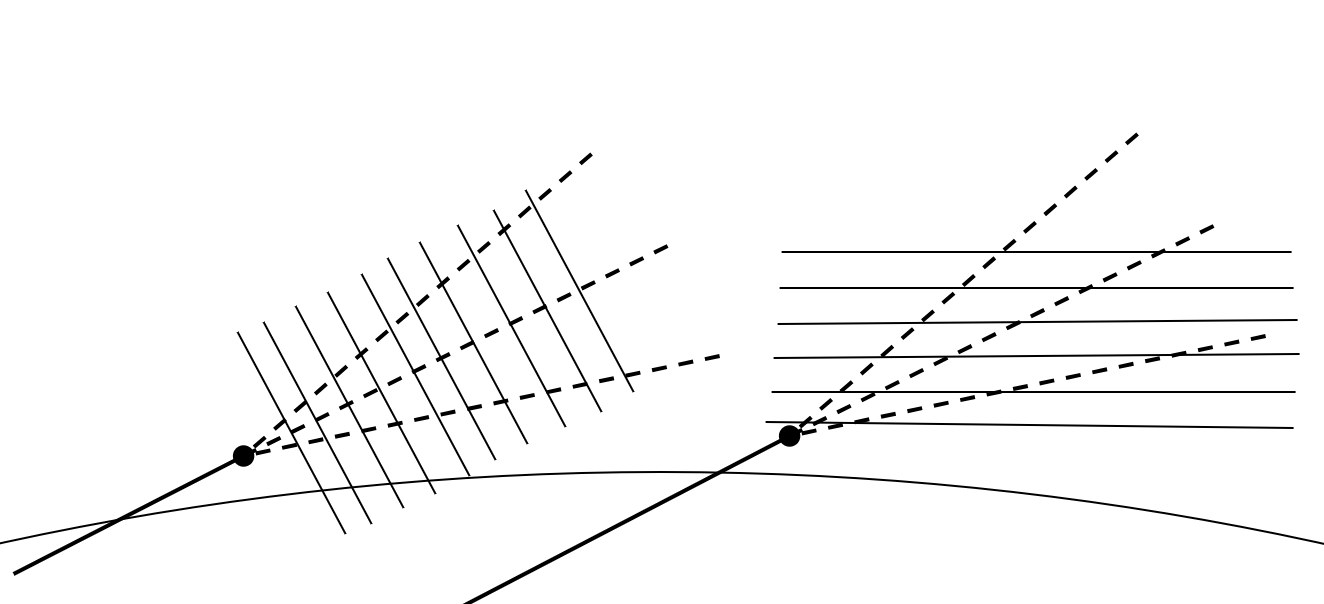
\includegraphics[width=.7\linewidth]{figures/cascadas/AIRES_planos}
		\caption{Disposiciones posibles de los niveles de observación en AIRES, en el ejemplo de una cascada hacia arriba. Izq.: A lo largo del eje del desarrollo. Der.: Dirección vertical.}
		\label{AIRES_planos}
	\end{figure}
	
Aunque presentaremos algún resultado con la configuración de la derecha en la Fig. anterior, normalmente optaremos por situar los niveles de observación a lo largo del eje del desarrollo\footnote{ Aunque a priori parezca irrelevante, la elección de niveles de observación tiene efectos no triviales en los valores obtenidos de la simulación, como comprobaremos en algún caso.}. Además, dado que conocemos el modelo atmosférico\footnote{ AIRES emplea la parametrización de Linsley.}, podremos convertir profundidad atravesada a altura o distancias \textit{recorridas} en la atmósfera aplicando \eqref{ec22}.

Teniendo en mente el funcionamiento de las simulaciones, podemos pasar a discutir el desarrollo de cascadas hacia arriba en la atmósfera. En primer lugar, presentaremos resultados de AIRES variando el ángulo de la cascada, la energía del primario y la altura de la primera interacción; y después haremos una comparativa entre cascadas de igual inclinación e iniciadas por el mismo primario, pero propagándose hacia arriba o hacia abajo.

	Cosas de Carac\_UG y Comp\_UGDG
	\clearpage %cleardoublepage pode meter paxinas en branco. Non e obrigatorio. Tampouco para a 
	\section{Emisión en radio: Principio físico y caracterización}\label{sec3}
	El objetivo fundamental de este trabajo, como hemos comentado en el apartado introductorio, es la caracterización de las radiofrecuencias emitidas en cascadas atmosféricas y el estudio de su posible aprovechamiento para la detección de neutrinos tau de origen astrofísico. Para poder avanzar en esta cuestión, primero presentaremos los mecanismos físicos que originan dicha emisión, ya que una buena comprensión de los mismos es, como poco, importante para poder interpretar los resultados posteriores.
	\subsection{Formalismo de la emisión}\label{sec31}
	Como es bien sabido, la presencia de cargas en movimiento en un determinado medio implica, casi de manera inevitable, la emisión de radiación. Resulta entonces evidente que, en una cascada atmosférica iniciada, por ejemplo, por un protón o un neutrino de origen astrofísico en la que aparecerán un número gigantesco de partículas cargadas propagándose con una velocidad $v\sim c$, podemos esperar la aparición de radiación electromagnética.
	
	Ahora bien, uno podría pensar a priori que, en las escalas de energía y número de partículas que involucra una cascada atmosférica, el balance \textit{macroscópico} de cargas positivas y negativas debería ser nulo, y por lo tanto las respectivas contribuciones a la radiación electromagnética emitida deberían cancelarse. Sin embargo, existen dos aspectos acerca del desarrollo de una cascada en la atmósfera que inmediatamente nos obligan a abandonar esta perspectiva ingenua:
	\begin{itemize}
		\item En primer lugar, la cascada se desarrolla en presencia del campo magnético terrestre, y por lo tanto las cargas sufren una deflexión en un sentido u otro según el signo de su carga. En una perspectiva \textit{macroscópica}, podemos interpretar que este efecto origina una corriente neta perpendicular tanto al desarrollo de la cascada como al campo magnético terrestre, generando entonces un campo eléctrico.
		\item En segundo lugar, la cascada no se desarrolla en el vacío sino en presencia de materia. Aunque en la cascada se produzca globalmente el mismo número de partículas con carga positiva que negativa, las interacciones con el medio darán lugar a un exceso de carga. Por ejemplo, los positrones generados en la cascada sufrirán procesos de aniquilación con los electrones del medio. Por otra parte, estos mismos electrones del medio podrán ser extraídos por diversos procesos (scattering $e^-e^-$, difusión Compton, ...) y contribuirán también a la aparición de una corriente neta. 
	\end{itemize}

Estos dos mecanismos, a los que a partir de ahora nos referiremos como \textit{deflexión geomagnética} y \textit{efecto Askaryan}\footnote{ Este mecanismo de emisión fue propuesto por Gurgen A. Askaryan en la década de los 60.} respectivamente, serán los procesos que darán lugar fundamentalmente a la emisión coherente de radiación electromagnética en cascadas atmosféricas.

Para ahondar en los mecanismos de emisión, recordaremos brevemente algunos conceptos de la electrodinámica clásica que nos permitirán explicar, al menos de manera cualitativa, los campos eléctricos que esperamos a partir de cada mecanismo. Partiremos de las ecuaciones de Maxwell en términos de los potenciales:
	\begin{equation}
	\vect{\nabla}^2\phi+\frac{\partial}{\partial t}\left(\vect{\nabla}\cdot\vect{A}\right)=-\frac{\rho}{\varepsilon}\label{ec31}
	\end{equation}
	\begin{equation}
	\vect{\nabla}^2\vect{A}-\mu\varepsilon\frac{\partial^2\vect{A}}{\partial t^2}-\vect{\nabla}\left(\vect{\nabla}\cdot\vect{A}+\mu\varepsilon\frac{\partial^2\phi}{\partial t^2}\right)=-\mu\vect{J}\label{ec32}
	\end{equation}

Por la libertad gauge, escogemos $\vect{\nabla}\cdot \vect{A}=0$ (gauge de Coulomb). En ese caso, los potenciales electromagnéticos toman la forma\footnote{ Véase por ejemplo \cite{Jackson2002}.} ($\vect{R}=\vect{r}-\vect{r}'$):
\begin{equation}
	\phi(\vect{r}, t)=\frac{1}{4\pi\varepsilon}\int_{\text{fuente}} \frac{\rho(\vect{r}', t)}{\left|\vect{R}\right|}d^3r'\label{ec33}
\end{equation}
\begin{equation}
	\vect{A}\left(\vect{r}, t\right)=\frac{\mu}{4\pi}\int_{\text{fuente}}\frac{\left[\vect{J}\left(\vect{r}', t_{ret}\right)-\left(\vect{J}\left(\vect{r}', t_{ret}\right)\cdot \hat{\vect{R}}\right)\hat{\vect{R}}\right]}{\left|\vect{R}\right|}d^3r'+\mathcal{O}(\left|\vect{R}\right|^{-3})\label{ec34}
\end{equation}
donde\footnote{ $n$ es el índice de refracción del medio.} $t_{ret}=t-nR/c$, y en \eqref{ec34} se desprecian términos que no contribuyen en la región de radiación. Las expresiones anteriores, aunque no sean especialmente simples de manejar, nos permitirán caracterizar los dos mecanismos de emisión que hemos comentado, sin más que tener en cuenta que:
\begin{itemize}
	\item En este gauge, el potencial escalar $\phi$ viene dado por una solución \textit{instantánea}, en el sentido de que no hay ninguna dependencia con $t_{ret}$. La consecuencia inmediata es que $\phi$ sólo describe efectos de campo cercano, y podremos escribir sencillamente:
	\begin{equation}
		\vect{E}=-\vect{\nabla}\phi-\dot{\vect{A}}\implies \vect{E}_{rad} = -\dot{\vect{A}}\label{ec35}
	\end{equation}
\item La solución para el potencial vector depende exclusivamente de la componente \textit{perpendicular} a $\vect{R}$ de la corriente:
\begin{equation}
	\vect{J}=\vect{J}_\parallel+\vect{J}_\perp = \left(\vect{J}\cdot\hat{\vect{R}}\right)\hat{\vect{R}}-\hat{\vect{R}}\times\left(\hat{\vect{R}}\times\vect{J}\right)\label{ec36}
\end{equation} 
Por lo tanto, el breve desarrollo anterior nos permite establecer que el campo eléctrico radiado tendrá la dirección de la componente perpendicular $\vect{J}_\perp$ de la corriente generada por cada mecanismo:
\begin{equation}
	\left.
	\begin{array}{c}
		\vect{E}_{rad} = -\dot{\vect{A}}\\
		\vect{A}\sim\vect{J}_\perp=-\hat{\vect{R}}\times\left(\hat{\vect{R}}\times\vect{J}\right)
	\end{array}
\right\}\vect{E}_{rad}\parallel  \hat{\vect{R}}\times\left(\hat{\vect{R}}\times\vect{J}\right)\label{ec37}
\end{equation}
\end{itemize}
Este último resultado es suficiente para estudiar la polarización del campo eléctrico generado por una cascada atmosférica, bien por deflexión geomagnética o por efecto Askaryan. Por simplicidad, consideremos una cascada que se desarrolla en la dirección vertical (i.e. con un ángulo cenital $\theta=0$). El efecto de la deflexión geomagnética está determinado por la acción de la fuerza de Lorentz sobre las cargas generadas:
\begin{equation}
	\vect{F}=q\vect{v}\times \vect{B}\implies \vect{J}\sim \hat{\vect{n}}_{\text{shower}}\times\vect{B}\label{ec38}
\end{equation}
donde $\hat{\vect{n}}_{\text{shower}}$ representa la dirección del desarrollo de la cascada. El efecto puede verse más claramente en la Fig. \ref{Geomag_deflexion}, en donde también representamos la polarización del campo radiado mediante este mecanismo.

\newpage
\begin{figure}[H]
	\centering
	\subfigure[]{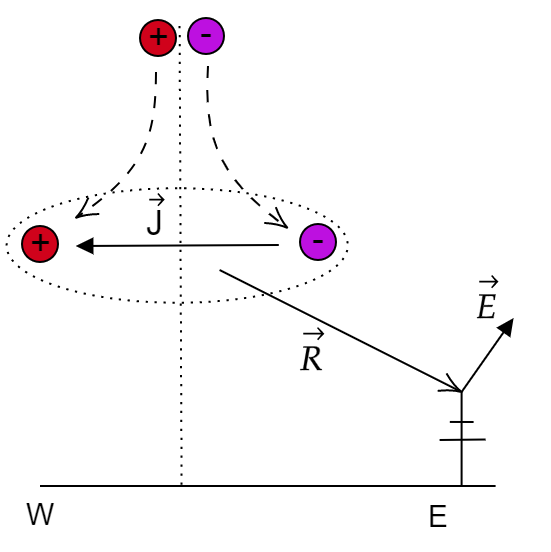
\includegraphics[width=0.3\linewidth]{figures/Geomag_deflexion_1}}
	\hspace{10mm}
	\subfigure[]{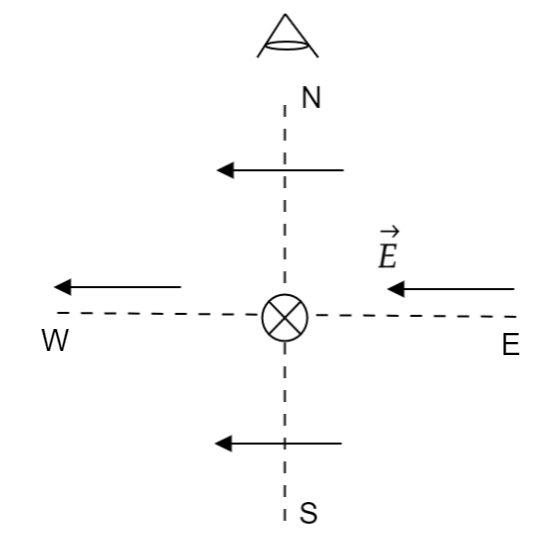
\includegraphics[width=0.3\linewidth]{figures/Geomag_deflexion_2}}
	\caption{Campo eléctrico radiado por efecto de la deflexión geomagnética. (a) Dirección del campo $\vect{E}_{rad}\parallel  \hat{\vect{R}}\times\left(\hat{\vect{R}}\times\vect{J}\right)$ en una antena prueba al este de una cascada vertical. (b) Dirección esperada para el campo eléctrico radiado en una cascada vertical (se indica la posición del observador de la fig. a). Las direcciones N, S, E, W hacen referencia al polo norte magnético.}
	\label{Geomag_deflexion}
\end{figure}

Si queremos hacer el mismo análisis para el efecto Askaryan, la polarización del campo radiado ahora estará determinada por el exceso de carga que aparece a lo largo del desarrollo. Naturalmente, las partículas más abundantes en una cascada atmosférica serán electrones y positrones, tanto por ser las especies de menor masa como por existir numerosos mecanismos que los originan. Como ya mencionamos, los positrones desaparecerán en procesos de aniquilación, mientras que otros electrones del medio serán extraídos y contribuirán a la carga neta generada. Por ello, el efecto Askaryan se traduce en la aparición de un exceso de carga negativa a lo largo del desarrollo y por tanto:
\begin{equation}
	\vect{J}\sim -\hat{\vect{n}}_{\text{shower}}\label{ec39}
\end{equation}
La polarización del campo generado por este mecanismo se representa en la Fig. \ref{Askaryan} para una cascada vertical. Como vemos, expresiones sencillas como \eqref{ec37}, \eqref{ec38} y \eqref{ec39} son suficientes para describir cualitativamente el campo eléctrico radiado por una cascada de dirección arbitraria.
\begin{figure}[H]
	\centering
	\subfigure[]{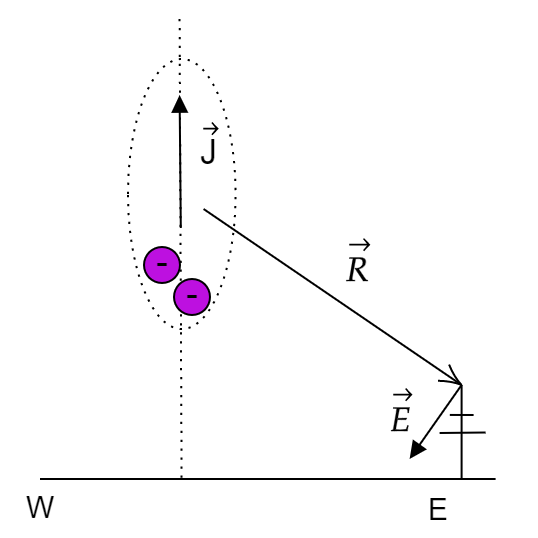
\includegraphics[width=0.3\linewidth]{figures/Askaryan_1}}
	\hspace{10mm}
	\subfigure[]{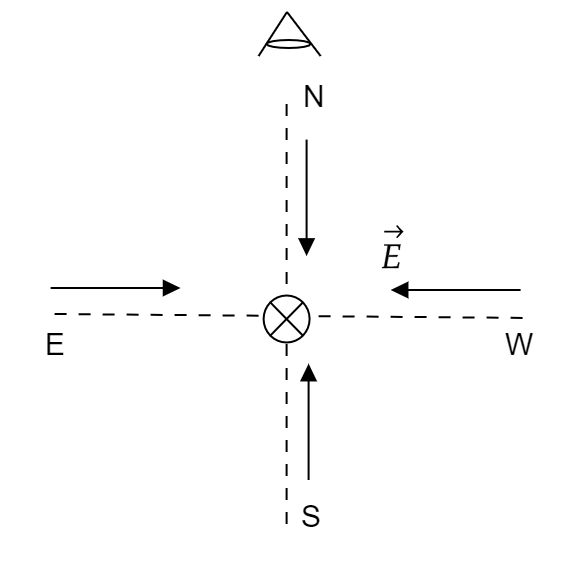
\includegraphics[width=0.3\linewidth]{figures/Askaryan_2}}
	\caption{Campo eléctrico radiado por efecto Askaryan. Mismos gráficos que en la Fig \ref{Geomag_deflexion}.}
	\label{Askaryan}
\end{figure}

Hasta ahora, hemos hecho una descripción \textit{macroscópica} de la emisión de radiación electromagnética, en el sentido de que hemos considerado la aparición de corrientes netas como un efecto global sobre la cascada. Aunque este enfoque es muy intuitivo y permite explorar las características de la emisión, un análisis detallado de la misma deberá realizarse desde una perspectiva \textit{microscópica}, i.e. considerando la radiación emitida por partículas cargadas de manera \textit{individual}. Dado que este es el marco en el que se desarrollan nuestras simulaciones, y también porque nos permitirá extraer alguna conclusión extra acerca de la emisión, estudiaremos algo más esta perspectiva. Para empezar, reescribamos el potencial vector \eqref{ec34}:
\begin{equation}
	\vect{A}\left(\vect{r}, t\right)=\frac{\mu}{4\pi}\int \frac{\vect{J}_\perp\left(\vect{r}', t'\right)}{\left|\vect{R}\right|}\,\delta\left(\frac{n}{c}\left|\vect{R}\right|-\left(t-t'\right)\right)d^3r'dt'\label{ec310}
\end{equation} 
donde sólo hemos introducido una función-$\delta$ que evalúa la corriente en $t_{ret}$. Supongamos ahora una carga puntual $q$ que se mueve a velocidad constante $\vect{v}$, entre $t=t_1$ y $t=t_2$. La corriente $\vect{J}$ asociada puede escribirse fácilmente:
\begin{equation}
	\vect{J}_\perp\left(\vect{r'}, t'\right)=q\vect{v}_\perp \,\delta^{(3)}\left(\vect{r}'-\vect{r}_0-\vect{v}t'\right)\left[\Theta\left(t'-t_1\right)-\Theta\left(t'-t_2\right)\right]\label{ec311}
\end{equation}
donde $\vect{r}_0=\vect{r}'\left(t=0\right)$, y el último término son funciones de Heaviside que garantizan que $\vect{J}_\perp=0$ para $t<t_1$ ó $t>t_2$. Sustituyendo esta última expresión en \eqref{ec310} e integrando en $d^3r'$ (aplicando la función-$\delta^{(3)}$), tenemos que:
\begin{equation}
	\vect{A}\left(\vect{r}, t\right)=\frac{\mu q}{4\pi}\vect{v}_\perp\int \frac{\delta\left(\frac{n}{c} \left|\vect{r}-\vect{r}_0-\vect{v}t'\right|-\left(t-t'\right)\right)}{\left|\vect{r}-\vect{r}_0-\vect{v}t'\right|}\left[\Theta\left(t'-t_1\right)-\Theta\left(t'-t_2\right)\right]dt'\label{ec312}
\end{equation}
A grandes distancias, en el régimen de Fraunhofer, podemos escribir:
\begin{equation}
	\left|\vect{r}-\vect{r}_0-\vect{v}t'\right|\approx R-t'\vect{v}\cdot\hat{\vect{R}}\;\;;\;\;\frac{1}{\left|\vect{r}-\vect{r}_0-\vect{v}t'\right|} \approx \frac{1}{R}\label{ec313}
\end{equation}
Sustituyendo estas aproximaciones en \eqref{ec312} y aplicando propiedades de las funciones $\delta$ y $\Theta$, es fácil obtener:
\begin{equation}
	\vect{A}\left(\vect{r}, t\right)\approx\frac{\mu q}{4\pi R}\vect{v}_\perp\frac{\Theta\left[t-nR/c-\left(1-n\beta\cos{\theta}\right)t_1\right]-\Theta\left[t-nR/c-\left(1-n\beta\cos{\theta}\right)t_2\right]}{1-n\beta\cos{\theta}}\label{ec314}
\end{equation}
donde hemos usado que $\left|\vect{v}\right|=\beta c$, además de definir el ángulo de observación como $\cos{\theta}=\hat{\vect{v}}\cdot\hat{\vect{R}}$. Como comentamos anteriormente, el campo eléctrico en este régimen puede obtenerse derivando \eqref{ec314} respecto a $t$:
\begin{equation}
	\vect{E}\left(\vect{r}, t\right)\approx-\frac{\mu q}{4\pi R}\vect{v}_\perp\frac{\delta\left[t-nR/c-\left(1-n\beta\cos{\theta}\right)t_1\right]-\delta\left[t-nR/c-\left(1-n\beta\cos{\theta}\right)t_2\right]}{1-n\beta\cos{\theta}}\label{ec315}
\end{equation}

De lo anterior puede extraerse la expresión para el campo eléctrico en el dominio de frecuencias, sin más que hacer una transformada de Fourier\footnote{ Se ha usado el criterio (poco común) de transformada de Fourier empleado en el algoritmo ZHS (ver siguiente apartado):
	$$\tilde{f}(\omega)=2\int dt \exp\left(i\omega t\right)f(t)$$}:
\begin{equation}
	\vect{E}\left(\vect{r}, \omega\right)\approx-\frac{\mu q}{2\pi R}\vect{v}_\perp \exp\left(i\omega\frac{nR}{c}\right)\frac{e^{i\omega(1-n\beta\cos{\theta})t_1}-e^{i\omega(1-n\beta\cos{\theta})t_2}}{1-n\beta\cos{\theta}}\label{ec316}
\end{equation}
Podríamos preocuparnos acerca del hecho de que lo que hemos obtenido es el campo eléctrico radiado por una partícula moviéndose a $\vect{v}$ constante, i.e., sin aceleración. Sin embargo, las funciones-$\delta$ de la expresión anterior implican que sólo existe una contribución no nula en los extremos de la trayectoria (recordemos que la partícula \textit{aparece} en $t_1$ y \textit{desaparece} en $t_2$, véase la ec. \ref{ec311}), mientras que a lo largo de la trayectoria no se emite radiación, como esperaríamos.

Más allá del comentario anterior, podemos extraer dos conclusiones importantes en lo que sigue:
\begin{itemize}
	\item En primer lugar, el campo eléctrico presenta una divergencia cuando el ángulo de observación coincide con el ángulo \v{C}erenkov del medio, $\cos{\theta_C}=1/n\beta$. Aunque esta divergencia es fruto de las aproximaciones del cálculo, describe correctamente el hecho de que el \textit{pico} de las emisiones se localiza en $\theta=\theta_C$. El resultado es natural, en una cascada se producirán partículas viajando a $v\sim c$, más rápido que la luz en la atmósfera ($n\geq 1$) y por lo tanto e valor máximo del campo eléctrico radiado aparecerá asociado al cono \v{C}erenkov.
	\item En segundo lugar, y desde un punto de vista más técnico, las expresiones \eqref{ec315} y \eqref{ec316} pueden incorporarse fácilmente a cálculos numéricos y simulaciones del desarrollo de cascadas.
\end{itemize}

Precisamente el último punto resulta de especial interés en este trabajo, ya que nuestro último objetivo será caracterizar la emisión de radio en cascadas atmosféricas hacia arriba mediante simulaciones. En el siguiente apartado nos detendremos en el algoritmo empleado en las mismas, y mostraremos algunos resultados sencillos que nos permitirán poner en contexto el desarrollo que hemos realizado en este apartado.

	\subsection{Simulación y caracterización de la radiación}\label{sec32}

Las simulaciones de la emisión electromagnética asociada a cascadas atmosféricas se ha realizado recurriendo al código ZHAireS \cite{AlvarezMuniz2012}, que combina la simulación del desarrollo de cascadas atmosféricas mediante AIRES con el algoritmo ZHS para calcular el campo eléctrico radiado. El desarrollo de la sección anterior será suficiente para describir, al menos de manera cualitativa, el funcionamiento de dicho algoritmo:
	\begin{itemize}
		\item Las trayectorias de las partículas son discretizadas en \textit{sectores}, en los cuales la velocidad de la partícula se toma constante.. Los parámetros de cada sector (energía, dirección, ...) se obtienen de AIRES.
		\item En cada paso de la simulación, la partícula se propagará a lo largo de un \textit{sector}, entre $t$ y $t+\Delta t$. Introduciendo las posiciones de observación (antenas) en la simulación, las expresiones \eqref{ec315} y \eqref{ec316} permiten calcular el campo eléctrico asociado al sector, tanto en dominio temporal como de frecuencias.
		\item Si en algún sector no se verifican las condiciones del régimen de Fraunhofer (e.g. trayectorias muy cercanas a una antena), dicho sector podrá subdividirse en \textit{subsectores} hasta alcanzar dimensiones lo suficientemente pequeñas para poder aplicar las expresiones \eqref{ec315} y \eqref{ec316}.
		%En cascadas atmosféricas, las dimensiones típicas de las mismas son comparables a la distancia a las antenas ($\sim 10^{2-3}\,\mathrm{m}$). Para evitar abandonar el 

		
	\end{itemize}
Mediante esta técnica, puede simularse el campo eléctrico radiado por una cascada atmosférica en función del tiempo o la frecuencia, sin más que acumular la contribución de todos las partículas consideradas en cada paso de la simulación. Además, las expresiones \eqref{ec315} y \eqref{ec316} se extraen directamente de principios básicos, sin suponer un mecanismo de emisión u otro. Por ello, este algoritmo tiene inmediatamente en cuenta la emisión de radiación asociada a la (des)aparición de partículas cargadas en el medio y a las interacciones consideradas, así como efectos de interferencia al sumar las contribuciones de cada partícula. En la Fig. \ref{ZHSsketch} mostramos esta idea:  
	\begin{figure}[H]
		\centering
		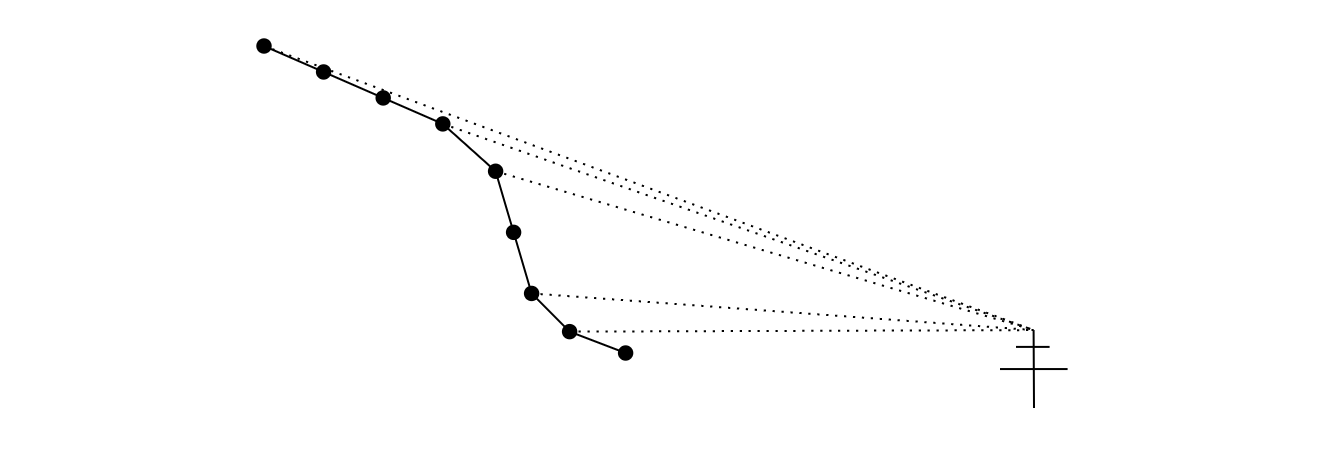
\includegraphics[width=.8\linewidth]{figures/ZHSsketch}
		\caption{Idea básica del algoritmo ZHS. La trayectoria de las partículas se discretiza, permitiendo aplicar expresiones como \eqref{ec315} de manera sencilla.}
		\label{ZHSsketch}
	\end{figure}
 
Mostraremos ahora algunos ejemplos de resultados típicos de ZHAireS, que nos permitirán poner de manifiesto algunas de las ideas desarrolladas hasta el momento. El primer caso que planteamos es el de una cascada vertical ($\theta=0$) iniciada por un protón de energía inicial $E=10^{17}\,\mathrm{eV}$. El campo magnético terrestre se ha supuesto, por simplicidad, horizontal (i.e., paralelo al plano del suelo) y de magnitud $23\,\mathrm{\mu T}$, y se han situado antenas en las cuatro direcciones relativas al \textit{core} de la cascada (N, S, E, W). Los resultados de la simulación se presentan en las Figs. \ref{EW_field} y \ref{NS_field}. Aunque a simple vista no es evidente, dichos resultados son un ejemplo perfecto para ver los efectos de los mecanismos de emisión que discutimos en la sec. \ref{sec31}. 

Empecemos por la Fig. \ref{EW_field}, en la que presentamos la componente $y$ del campo eléctrico, i.e., la componente en la dirección Este-Oeste (EW). Como vemos, la forma de la señal es muy similar en todas las posiciones, con un pulso de duración $\sim \mathrm{ns}$ cuya amplitud decrece con la distancia al \textit{core} de la cascada. Sin embargo, aparece una diferencia muy interesante en los máximos: tanto en las antenas al Norte y Sur se alcanzan los mismos valores aproximadamente, mientras que en las antenas al Este (Oeste) se llega a valores algo superiores (inferiores). En este efecto es donde podemos apreciar la competición entre la deflexión geomagnética y el efecto Askaryan. Recordando las Figs. \ref{Geomag_deflexion} y \ref{Askaryan}, es evidente que el efecto Askaryan no modifica de manera sustancial la componente $y$ del campo si nos situamos al Norte o al Sur, mientras que aporta una contribución que se añade (resta) al campo generado por deflexión geomagnética al Este (Oeste). Por ello, el campo observado en el Este es ligeramente superior al del Oeste, mientras que este efecto no aparece en observaciones al Norte o Sur.


\begin{figure}[H]
	\centering
	\subfigure[Norte]{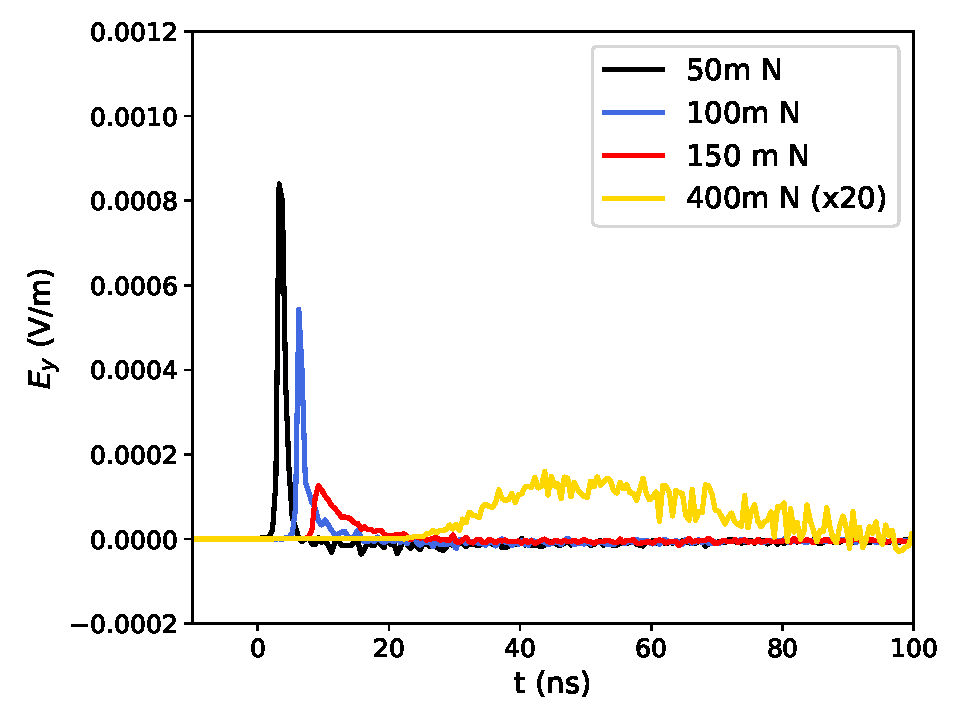
\includegraphics[width=0.45\linewidth]{figures/radio/p_1e17_0deg_EW_N}}
	\subfigure[Sur]{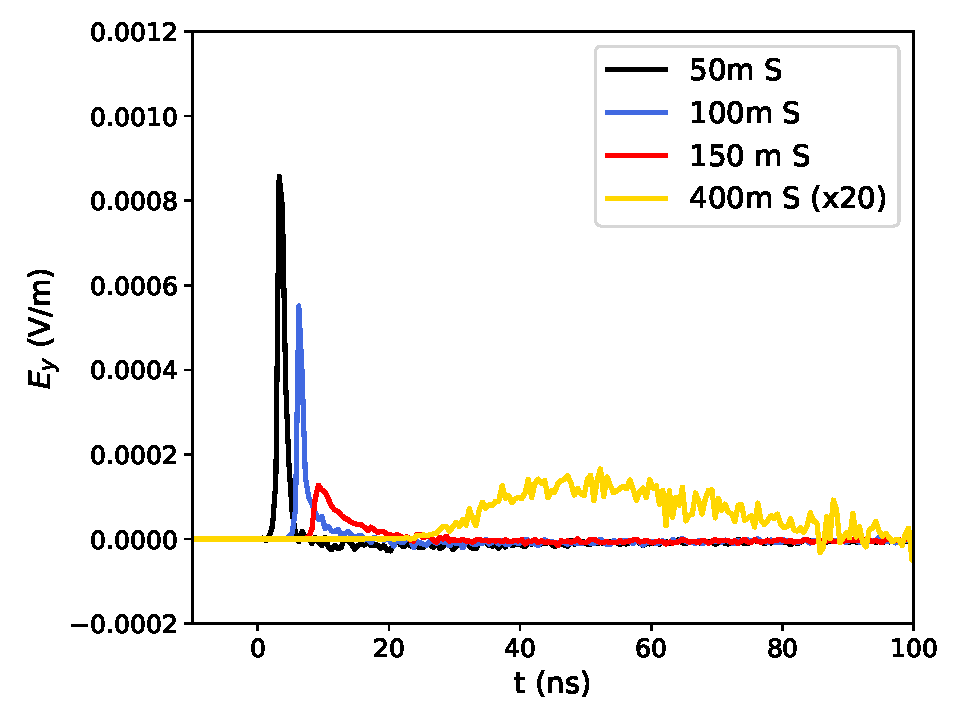
\includegraphics[width=0.45\linewidth]{figures/radio/p_1e17_0deg_EW_S}}
	\\
	\subfigure[Este]{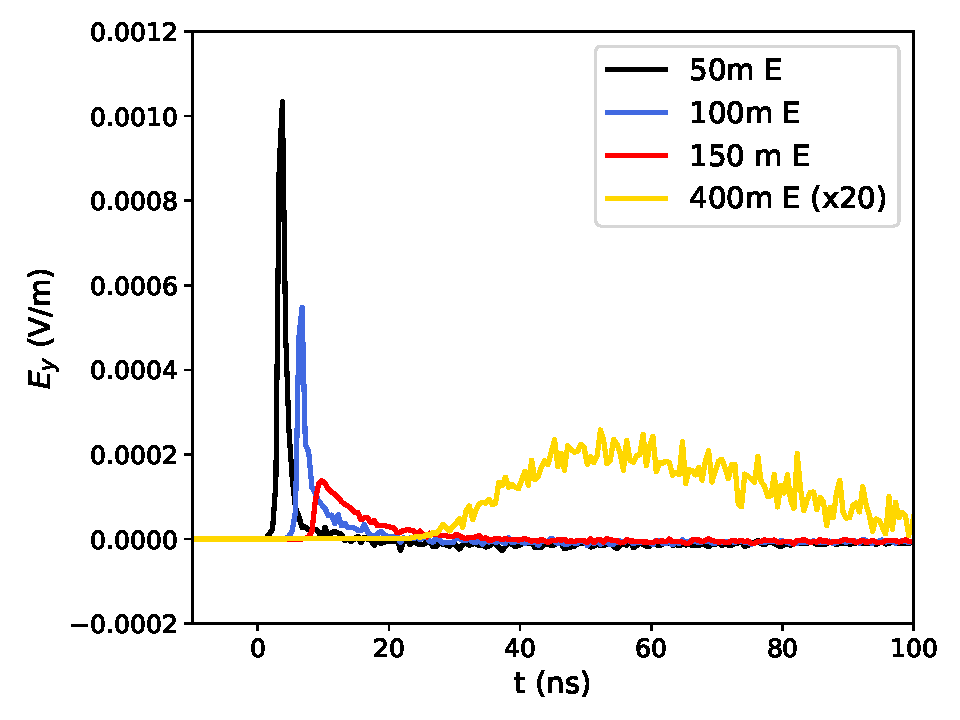
\includegraphics[width=0.45\linewidth]{figures/radio/p_1e17_0deg_EW_E}}
	\subfigure[Oeste]{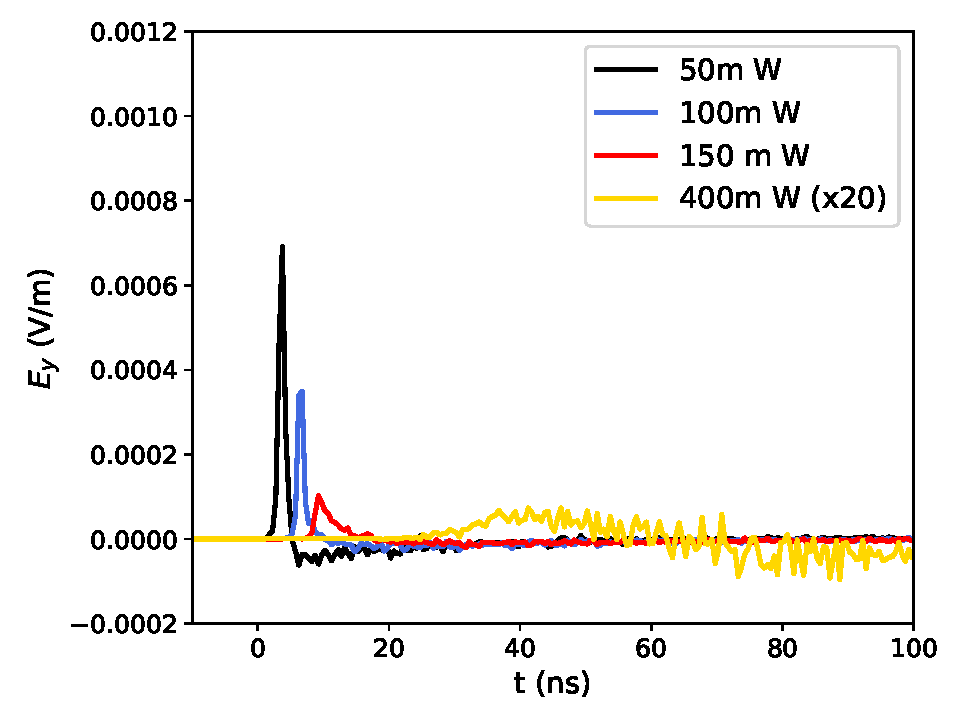
\includegraphics[width=0.45\linewidth]{figures/radio/p_1e17_0deg_EW_W}}
	\caption{Componente $y$ (E$\rightarrow$W) del campo eléctrico radiado por una cascada vertical iniciada por un protón de $10^{17}\,\mathrm{eV}$, en diferentes puntos de observación. La señal a $400\,\mathrm{m}$ se ha multiplicado por un factor $20$ para hacerla visible.}
	\label{EW_field}
\end{figure}

Si nos centramos en la componente $x$ del campo, es decir, en la dirección Norte-Sur (NS), es evidente a partir de las Figs. \ref{Geomag_deflexion} y \eqref{Askaryan} que sólo \textit{veremos} el efecto Askaryan en antenas al Norte y Sur, mientras que la deflexión geomagnética no será relevante. Además, esperamos que dicha componente NS del campo tenga signo opuesto. Precisamente, este es el resultado que observamos en la Fig. \ref{NS_field}. Además, por simetría (Fig. \ref{Askaryan}), podemos suponer que la amplitud del máximo de la componente $x$ del campo en antenas al N,S ($\sim 2\times10^{-4}\,\mathrm{V/m}$) será igual a la amplitud del máximo de la componente $y$ del campo en antenas al E,W.  vemos como los valores máximos que alcanza el campo eléctrico en este caso. Como vemos, dicho valor es plenamente coherente con que la diferencia que observábamos en las antenas E,W en la Fig. \ref{EW_field} tenga su origen en el efecto Askaryan.
\begin{figure}[H]
	\centering
	\subfigure[Norte]{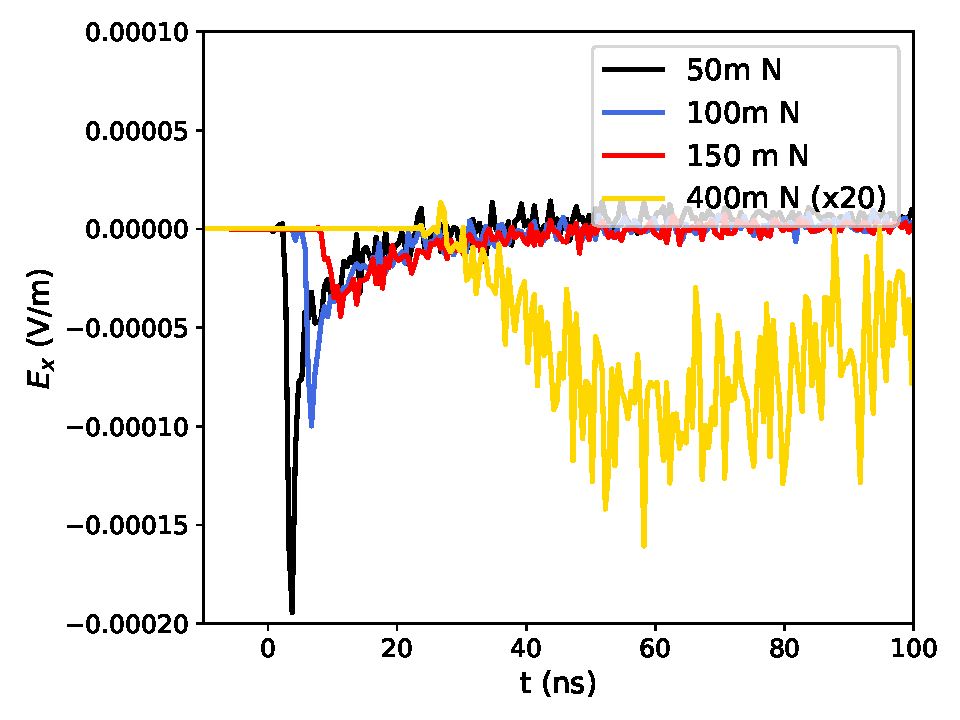
\includegraphics[width=0.45\linewidth]{figures/radio/p_1e17_0deg_NS_N}}
	\subfigure[Sur]{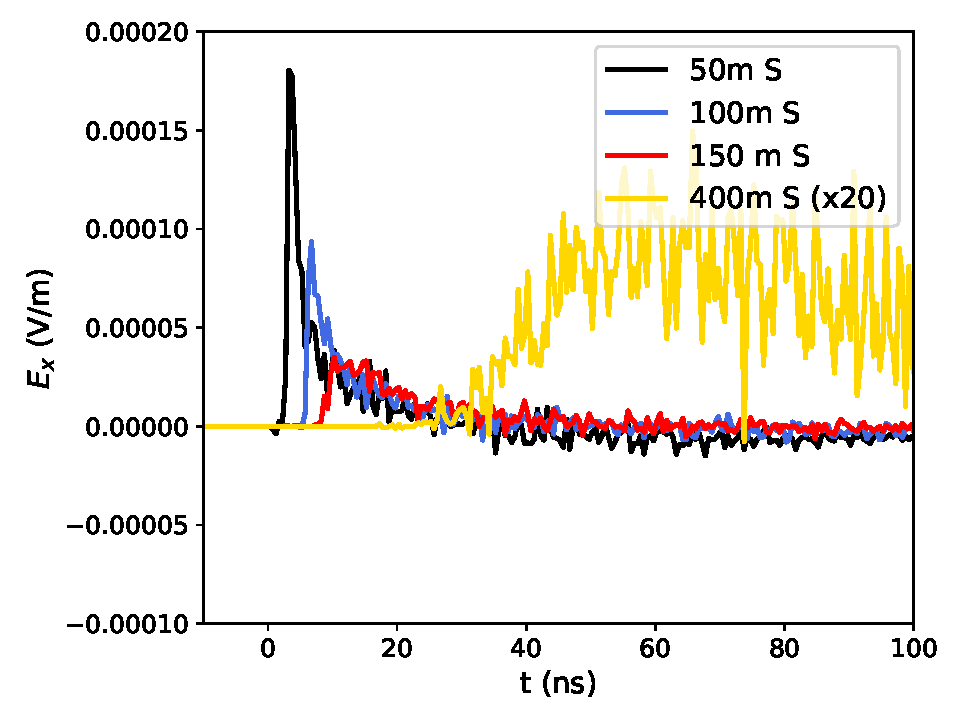
\includegraphics[width=0.45\linewidth]{figures/radio/p_1e17_0deg_NS_S}}
	\\
	\subfigure[Este]{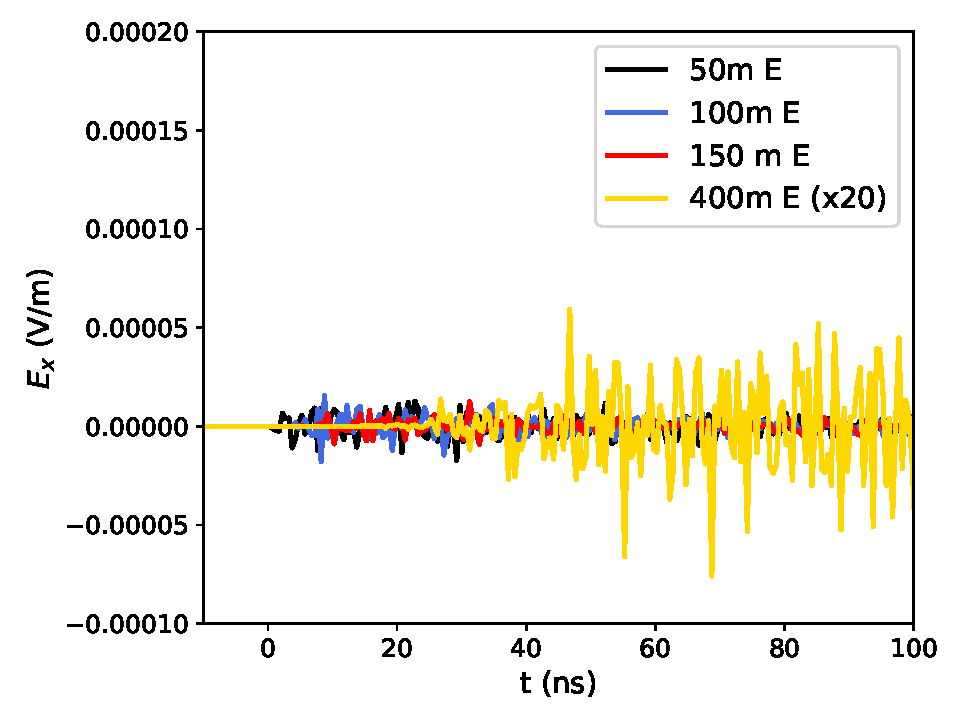
\includegraphics[width=0.45\linewidth]{figures/radio/p_1e17_0deg_NS_E}}
	\subfigure[Oeste]{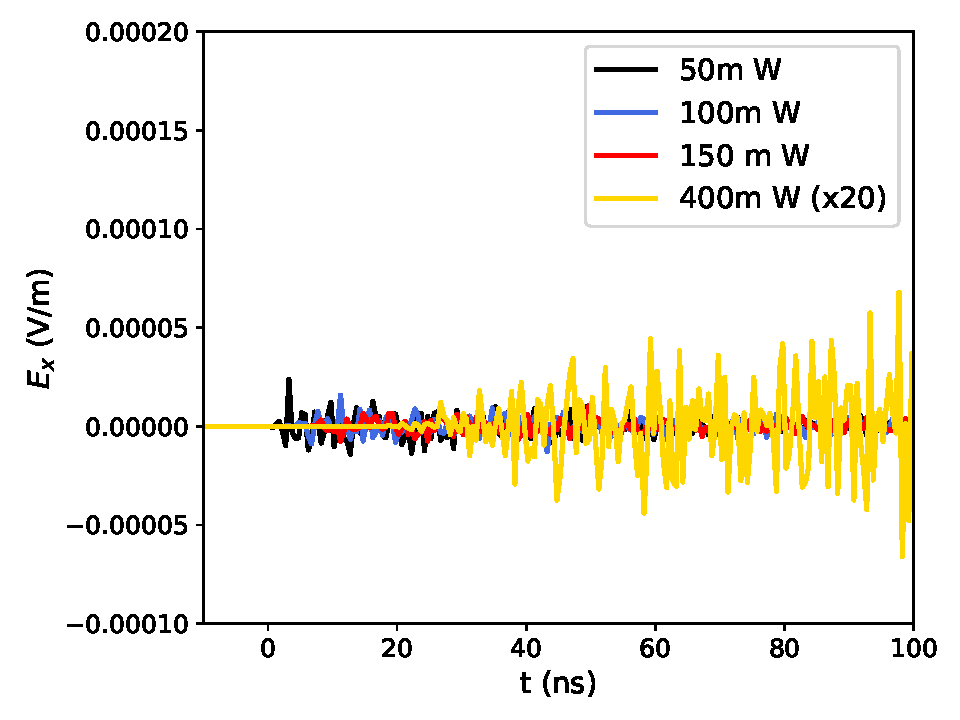
\includegraphics[width=0.45\linewidth]{figures/radio/p_1e17_0deg_NS_W}}
	\caption{Equivalente a Fig. \ref{EW_field} para la componente $x$ (S$\rightarrow$N) del campo.}
	\label{NS_field}
\end{figure}

El siguiente caso que plantearemos es el de una cascada inclinada, iniciada por una partícula primaria de mayor energía. Concretamente, se ha simulado una cascada iniciada por un protón de energía $E=10^{19}\,\mathrm{eV}$, con una trayectoria de ángulo cenital $\theta=70^{\circ}$. En este caso, se ha supuesto un campo magnético ligeramente diferente\footnote{ Concretamente, este campo magnético es similar al que se encuentra en el Polo Sur, una localización de especial interés experimental para el estudio de la radiación cósmica.}, de magnitud $55\,\mathrm{\mu T}$ y ángulo de inclinación $I = 72,42^\circ$; mientras que las antenas se han situado a lo largo de las direcciones NS y EW (Fig. \ref{ANITApaper_showscheme}). Esta configuración nos permitirá estudiar algo más en detalle el campo eléctrico observado en función de la distancia a la cascada.

Como mencionamos en el primer apartado de esta sección, el máximo de la emisión ocurre cuando el ángulo de observación coincide con el ángulo \v{C}erenkov. Por ello, en el suelo se registrará el máximo del campo eléctrico en las antenas que observen el máximo del desarrollo de la cascada bajo un ángulo $\theta_C$; ya que en la posición del máximo de la cascada es donde existe un mayor número de partículas, cuya radiación será la contribución dominante a toda la emisión. Por ello, el pico de $\vect{E}$ aparecerá en la intersección del suelo con el cono \v{C}erenkov, cuyo vértice se sitúa en el máximo de la cascada. 
\begin{figure}[H]
	\centering
	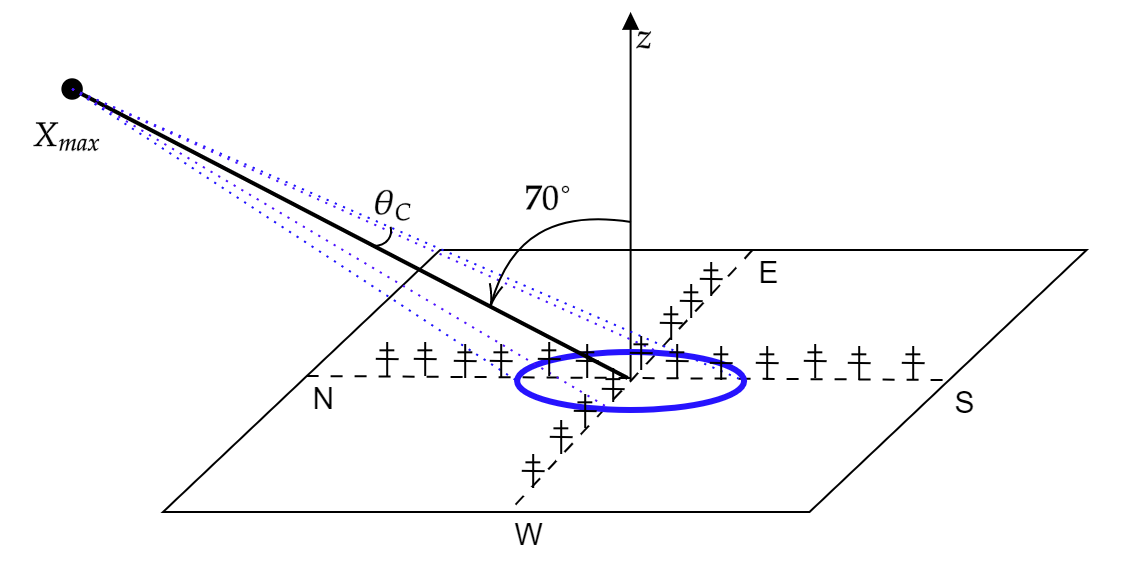
\includegraphics[width=.6\linewidth]{figures/radio/ANITApaper_showscheme}
	\caption{Configuración planteada. Se situaron 50 antenas a lo largo de cada eje, hasta $1500\,\mathrm{m}$ del \textit{core} de la cascada. El máximo de emisión se espera en la intersección del cono \v{C}erenkov con el suelo.}
	\label{ANITApaper_showscheme}
\end{figure}

Evidentemente, para una cascada inclinada la intersección del cono \v{C}erenkov con el suelo no será una circunferencia sino una elipse. Si para esta configuración representamos el máximo de la componente EW del campo eléctrico registrado en cada antena, obtenemos la siguiente figura:
\begin{figure}[H]
	\centering
	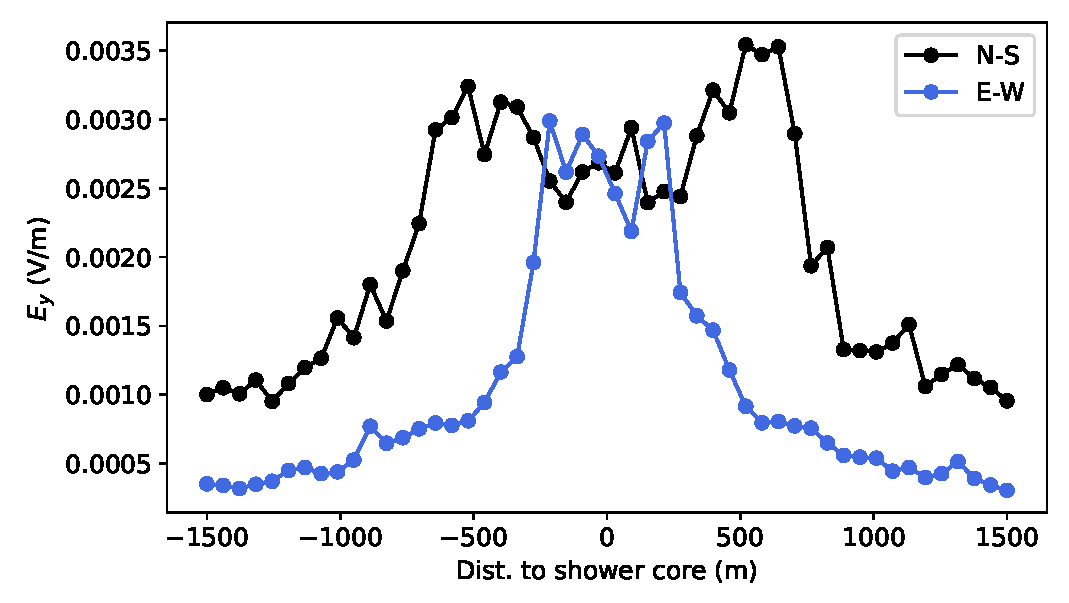
\includegraphics[width=.65\linewidth]{figures/radio/downgoing_p_10EeV_70deg_Ey_t_ground}
	\caption{Máximo del campo eléctrico registrado en las antenas a nivel del suelo de la configuración \ref{ANITApaper_showscheme}. Se representan los valores en los dos ejes (NS, EW).}
	\label{downgoing_p_10EeV_70deg_Ey_t_ground}
\end{figure}
El resultado no es especialmente esclarecedor, ya que esperaríamos dos máximos bien definidos a lo largo de los dos ejes. Si bien puede intuirse un comportamiento así en las antenas situadas a lo largo de la dirección NS, no ocurre así para la dirección EW.

Lo que haremos será estudiar el campo eléctrico en el dominio de frecuencias, en lugar de representar el máximo en tiempo como hemos hecho. Como ya mencionamos, ZHAireS permite obtener el espectro en frecuencia del campo eléctrico en cada antena. Antes de presentar los resultados que hemos obtenido de esta manera, haremos una breve digresión acerca de los valores de frecuencia que debemos considerar.

La estimación más rápida para las frecuencias asociada a la radiación electromagnética emitida puede hacerse a partir de los resultados \ref{EW_field} y \ref{NS_field}. Puesto que tiempo y frecuencia son variables conjugadas de Fourier, la duración de los pulsos nos da un orden de magnitud para $f$:
\begin{equation}
	\omega T = 2\pi f T \sim 1\implies f\sim \left(2\pi T\right)^{-1} \implies T \sim 1 \,\mathrm{ns} \leftrightarrow f \sim 100 \,\mathrm{MHz}\label{ec317}
\end{equation} 
Por lo tanto, podemos adelantar que las frecuencias de interés estarán en el rango de las radiofrecuencias ($\sim30\,\mathrm{MHz}-1\,\mathrm{GHz}$). Una razón para que la emisión relevante aparezca en esta banda de frecuencias puede verse con argumentos sencillos de coherencia, i.e., exigiendo que la longitud de onda sea comparable a las dimensiones de la cascada:
	\begin{figure}[H]
		\centering
		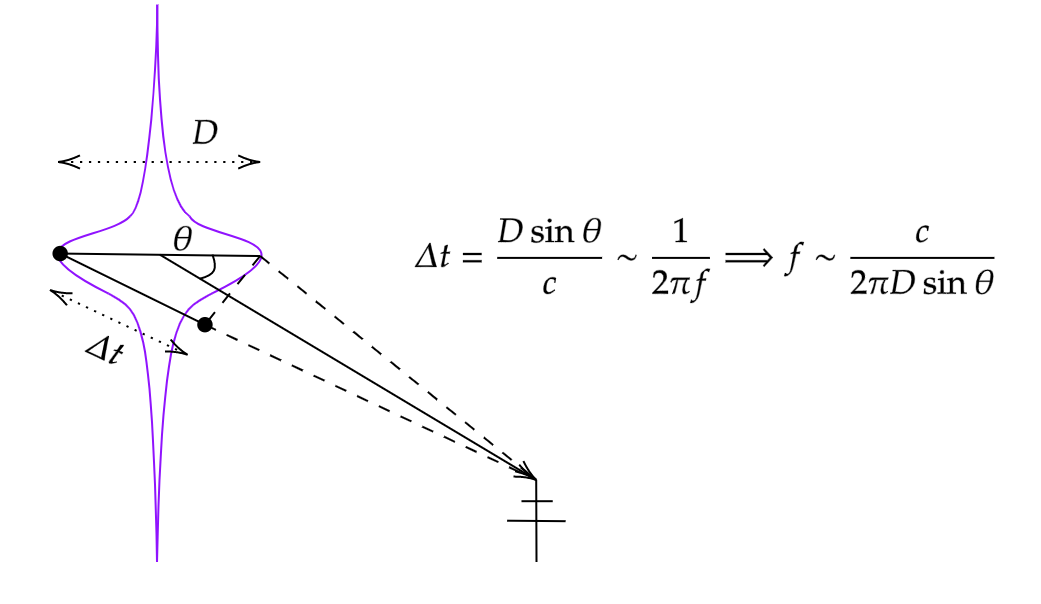
\includegraphics[width=.6\linewidth]{figures/radio/coherence}
		\caption{Geometría considerada. $D$ se corresponde con el desarrollo lateral de la cascada en el máximo.}
		\label{coherence}
	\end{figure}
Tomando valores típicos para una cascada en la atmósfera ($D\sim 100\,\mathrm{m}$, $\theta\sim\theta_C\sim1^\circ$), se encuentra $f\sim30\,\mathrm{MHz}$. Por lo tanto, debemos quedarnos con que los rangos de frecuencia que nos interesan son de radiofrecuencias.

Sabiendo lo anterior, presentamos en la Fig. \ref{freqfieldsgrounds} algunas componentes de Fourier obtenidas con la configuración de la Fig. \ref{ANITApaper_showscheme}. Como vemos en la primera gráfica, en este caso sí aparecen perfectamente definidos los máximos asociados al cono \v{C}erenkov, estando más separados en la dirección N-S como era de esperar, dada la inclinación de la cascada. La explicación para los resultados de la Fig. \ref{downgoing_p_10EeV_70deg_Ey_t_ground} puede extraerse de la gráfica de la derecha, en la que representamos las componentes de Fourier del campo a varias frecuencias. Como vemos la amplitud de las componentes decrece con la frecuencia\footnote{ Tomando el límite $\theta\rightarrow\theta_C$ de manera adecuada en \eqref{ec316} puede verse que $\vect{E}\left(\vect{r},\omega\right)\propto\omega$.}, aunque quizá el efecto más relevante es que la \textit{resolución} de los máximos decrece con la frecuencia, llegando a estar prácticamente superpuestos para las frecuencias más bajas. 

La explicación a este hecho puede encontrarse en fenómenos de tipo difractivo. Podemos ejemplificarlo recordando, e.g., el patrón de Airy, en el que el primer cero del patrón de difracción ocurre cuando, respecto al máximo, observamos bajo un ángulo $\alpha$ tal que:
\begin{equation}
	\sin\alpha=1,22\frac{\lambda}{d}\label{ec318}
\end{equation}  
donde $d$ es el tamaño típico de la fuente. Evidentemente, a menor (mayor) frecuencia (longitud de onda), debemos irnos hasta un mayor $\alpha$ para encontrar el mínimo del patrón. Es decir, cuanto menor sea la frecuencia mayor será la anchura del pico, como observamos en \ref{freqfieldsgrounds}b
\begin{figure}[H]
	\centering
	\subfigure[Componente a $300\,\mathrm{MHz}$]{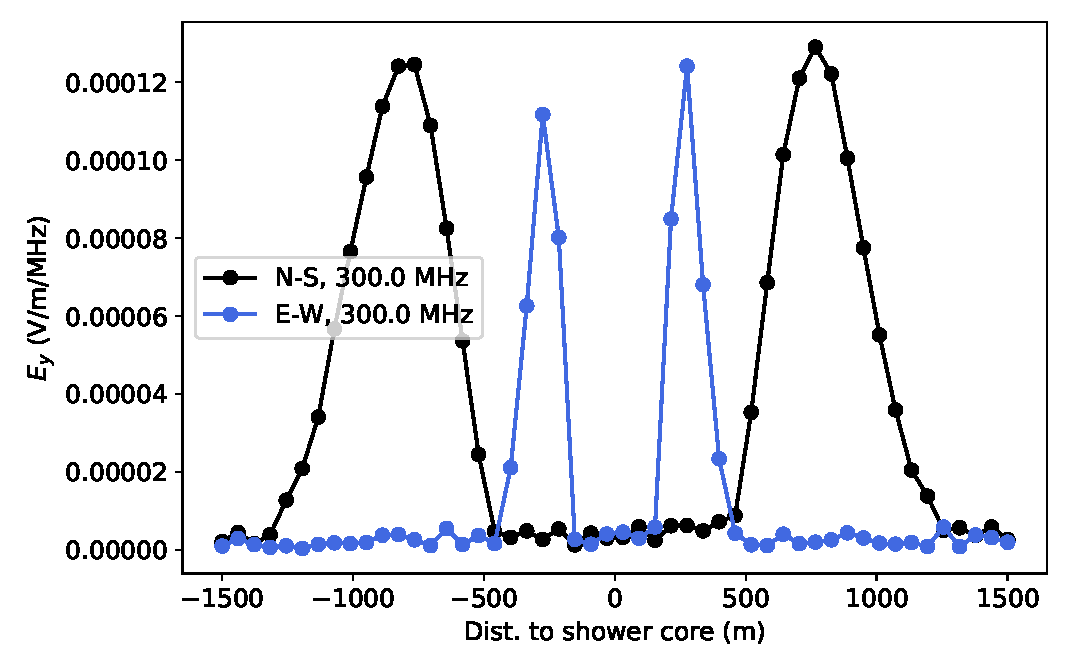
\includegraphics[width=0.49\linewidth]{figures/radio/downgoing_p_10EeV_70deg_Ey_300MHz_ground}}
	\subfigure[Componentes a varias frecuencias a lo largo de la dirección EW]{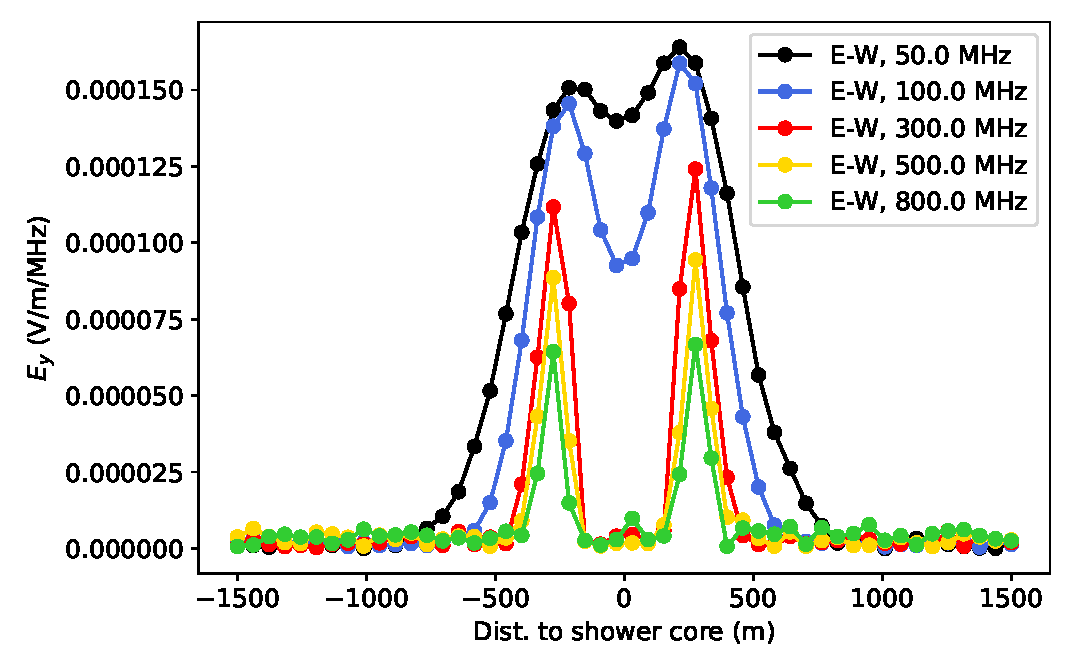
\includegraphics[width=0.49\linewidth]{figures/radio/downgoing_p_10EeV_70deg_Ey_varfreq_groundEW}}
	\caption{Componentes de Fourier del campo eléctrico (componente $y$) en función de la distancia al \textit{core} de la cascada.}
	\label{freqfieldsgrounds}
\end{figure} 
Evidentemente, en la Fig. \ref{downgoing_p_10EeV_70deg_Ey_t_ground} estábamos viendo la superposición de todas las componentes de Fourier, y debido a que las dominantes (baja frecuencia) no están resueltas, no se observaba claramente la intersección del cono \v{C}erenkov con el suelo.

Para acabar esta sección, recapitularemos los resultados y conclusiones más importantes:
\begin{enumerate}
	\item En cascadas atmosféricas tendremos dos contribuciones fundamentales a la emisión de radiación electromagnética: deflexión geomagnética y efecto Askaryan, cada una con efectos diferentes en la polarización del campo detectado.
	\item Las expresiones deducidas para el campo eléctrico radiado no asumen ningún mecanismo de emisión, y están integradas en el código ZHAireS empleado para realizar las simulaciones. Como hemos visto, el efecto de ambos mecanismos es evidente en los resultados.
	\item Las frecuencias de interés se sitúan en la banda de los $\mathrm{MHz}$ (radiofrecuencias). Además, la señal de campo eléctrico detectada tiene una dependencia importante con la frecuencia, tanto en amplitud (mayor a menores frecuencias) como en la resolución de los máximos en torno al ángulo \v{C}erenkov.
\end{enumerate}

	\clearpage

	\section{Emisión en radio en cascadas hacia arriba}
	\clearpage %cleardoublepage pode meter paxinas en branco. Non e obrigatorio. Tampouco para a 
	\section{Conclusiones}
	
	
	%%%%%%%Bibliografía
	\clearpage
	\appendix
	
	\markboth{REFERENCIAS}{REFERENCIAS}  
	\addcontentsline{toc}{section}{Referencias} 
	\nocite{*}
	\bibliography{TFMbib}
	\bibliographystyle{apalike}

	
\end{document}